
\documentclass{amsart}

\usepackage{graphicx}
%\usepackage[altbullet]{lucidabr}
%two lines below change font (font intalled manually (i.e. uploaded))
%\usepackage{fontspec}
%\setmainfont[Ligatures=TeX]{LucidaBrightRegular.ttf}
%\usepackage{kpfonts}    % for nice fonts
% option [light] for more aery documents
\usepackage{color}  %for color of references
\usepackage[dvipsnames]{xcolor} %for color of references
\usepackage{caption}
\usepackage{fancyhdr}
\usepackage[pagebackref,colorlinks, citecolor=BlueViolet,urlcolor=BlueViolet]{hyperref}
\hypersetup{colorlinks = BlueViolet, allcolors = BlueViolet}
\usepackage[nameinlink,noabbrev]{cleveref} 
\usepackage{natbib}
\usepackage{multicol}
\usepackage{multirow}
%\usepackage{lscape}
\usepackage{pdflscape}
\usepackage{amssymb}
\usepackage{geometry}
\usepackage{longtable}
\usepackage{colortbl}
\usepackage{dsfont}
\usepackage{bm}
\usepackage{mathtools}
\usepackage{pgf}
\usepackage{tikz}
\usepackage{soul}
\usepackage{tikz}
\usepackage{tikz,fullpage}
\usepackage{pgf}
\usepackage{tikz}
\usepackage{bbm} %for the indicator function
\usetikzlibrary{shapes.geometric, arrows} %to create flow charts
\usepackage{bold-extra} %for bold small caps in the title
\usepackage{dirtree} % to create lists as tree

%\renewcommand{\familydefault}{\sfdefault} %for the sans serif font

%AMS original setup for mathematical elements
\newtheorem{theorem}{Theorem}[section]
\newtheorem{lemma}[theorem]{Lemma}
\theoremstyle{definition}
\newtheorem{definition}[theorem]{Definition}
\newtheorem{example}[theorem]{Example}
\newtheorem{xca}[theorem]{Exercise}
\theoremstyle{remark}
\newtheorem{remark}[theorem]{Remark}
\numberwithin{equation}{section}

%    Absolute value notation
\newcommand{\abs}[1]{\lvert#1\rvert}

%    Blank box placeholder for figures (to avoid requiring any
%    particular graphics capabilities for printing this document).
\newcommand{\blankbox}[2]{%
  \parbox{\columnwidth}{\centering
%    Set fboxsep to 0 so that the actual size of the box will match the
%    given measurements more closely.
    \setlength{\fboxsep}{0pt}%
    \fbox{\raisebox{0pt}[#2]{\hspace{#1}}}%
  }%
}

%Tikz setup for a flow chart
\tikzstyle{modelblock} = [rectangle, rounded corners, minimum width=3cm, minimum height=1cm,text centered, draw=black, fill=white, text ragged]

\tikzstyle{arrow} = [thick,->,>=stealth]

\begin{document}

\title{EC534 - Referee Report}

%    Information for first author
\author{}
%\address{}
%\curraddr{}
%\email{a.dyevre@lse.ac.uk}
%\thanks{}

%    Information for second author
%\author{}
%\address{}
%\email{}
%\thanks{}

%    General info
%\subjclass[2000]{}

%\date{\today. First created October 19, 2019}

%\dedicatory{}
%\keywords{}

%\begin{abstract}

%\end{abstract}

\maketitle

\begin{center}
Student number: 201324680
\end{center}


\vspace{12pt}

I am refereeing ``The rise of Market Power and Macroeconomic implications'' (November 2019 version) by \textbf{Jan De Loecker}, \textbf{Jan Eeckhout} and \textbf{Gabriel Unger}. The paper is forthcoming in the \textit{Quarterly Journal of Economics}.

%% The correct journal style for \specialsection is all uppercase; a known bug
%% in amsart.cls prevents this, so input must be uppercase until it is fixed.
%\specialsection*{This is a Special Section Head}
%\specialsection*{THIS IS A SPECIAL SECTION HEAD}
%This is an example of a special section head%
%%%%%%%%%%%%%%%%%%%%%%%%%%%%%%%%%%%%%%%%%%%%%%%%%%%%%%%%%%%%%%%%%%%%%%%%
%\footnote{Here is an example of a footnote. Notice that this footnote text is running on so that it can stand as an example of how a footnote with separate paragraphs should be written.
%\par
%And here is the beginning of the second paragraph.}%
%%%%%%%%%%%%%%%%%%%%%%%%%%%%%%%%%%%%%%%%%%%%%%%%%%%%%%%%%%%%%%%%%%%%%%%%
\newpage 

\section*{Summary of the paper}

This paper is an ambitious empirical exercise attempting to document the rise in market power in the US. It uses a novel and micro-founded estimation strategy in conjunction with firm-level balance sheet data to show that aggregate markups were stable at around a fifth of marginal cost from 1955 to 1980, but increased to three fifth of marginal cost over 1980-2016. The rise in aggregate markups is driven by a combination of two trends: firstly the upper tail of the markup distribution has fattened, and secondly high markup firms have captured a larger share of sales. These effects account for 1/3 and 2/3 of the aggregate increase, respectively. The paper then relates the rise in markups to macroeconomic trends such as the fall in the labour and capital shares, the decline in business dynamism and the decline in geographical and firm-to-firm labour reallocation.\\

While the authors' investigation of the consequences of large markups on macro outcomes provides a useful motivation for their empirical exercise, their main contribution is methodological. The authors uses data on publicly listed firms and on the universe of firms observed in the US Manufacturing, Retail and Wholesale Censuses to support their argument. Importantly, this version of the paper addresses several criticisms related to what this new markup measure may capture beyond market power, such as a rise in fixed costs, a rise in output elasticity or a rise in the share of marketing and advertising expenses in total expenditures.\\

The following section stresses the relevance of the paper for some central debates in macroeconomics. The section after it summarises my main comments about the paper. The last section concludes and the appendix provides a summary of the method used by the authors to estimate firm-level markups.

\section*{Relevance}

The paper's relevance cannot be overstated. A rise in markups can provide a unified explanation to several secular trends in macroeconomics whose causes remain the subjects of intense debates: (i) the fall in labour income, (ii) the decline in low-skill wages, (iii) the decline in labour force participation, (iv) the decline in geographical and inter-firm mobility, (v) and the slowdown in productivity growth. Irrespective of the solidity of the empirical evidence, a single unified explanation for all these phenomena is worthy of attention. While the authors remain agnostic about the causes of rising market power, simply showing long-term trends in markups is of central importance to the macroeconomics literature.\\

The paper's contribution is also important for the Industrial Organisation literature on market power and firm-level markup estimation. IO scholars had estimated sector- or firm-specific markups before, but cross-sector aggregate markup measures based on firm-level data has been a very recent endeavour. Moreover, the time-coverage of the paper is unmatched, making it a reference point for the study of long-term trends in markups


\section*{Major comments}

The paper opens itself to two types of criticisms: methodological and theoretical. The methodological concerns are about aggregation of firm-level markups, how the share of variable inputs is calculated and the relevance of their sample. The theoretical concerns are related to the link between the estimated rise in markups and the secular trends. As the empirical part of the paper is the most important contribution I dedicate more space to the methodological concerns.

\subsection*{Methodological concerns}

\subsubsection*{1. Aggregation} The authors use the sales share of firms to compute their headline measure of weighted average of markups in the American economy.\footnote{The authors defend this assumption by invoking the three following reasons: as reallocation of sales toward high-markup firms seems to be the driving force behind rising aggregate market power using input shares as weights would miss this trend, profits rates are aggregated with sales shares, and revenue weighting is used in the calculation of macroeconomic indicators such as GDP.} This choice is not innocuous. Markets are heterogeneous in a number of dimensions and competition plays out differently in different markets. Some are subject to high entry costs (airlines), some have become less  competitive due to regulatory capture (broadband and communications), and some have been prone to collusion (chemicals). IO economists have always been sceptical of aggregating measures of market power across industries. This methodological concern is a consequence of the authors' decision not to take a stance on the causes of rising market power. More justification about why it is acceptable to use sales shares as weights would have been welcome.\\

%\subsection*{Comparison with the evolution of industry-level markups}. A welcome addition to the most recent version of the paper consists of the comparison of the DLEU results with those of \cite{hall2018new}. The reason why industry-level markups do not experience as high a rise is Jensen's inequality.

Simple tweaks in weights can dramatically affect the level and growth of markups estimated by De Loecker and co-authors. One graph that did not survive in the latest version of the paper shows just how important this choice is. In the 2017 NBER working paper version, the authors find that the sales-share-weighted average of markups is actually lower than the unweighted average. See figure \ref{fig:unweighted} below. This is counter-intuitive as one would expect the weighted average to be larger than the unweighted one if high-markup firms are also those with the largest sales share. This would be consistent with the theoretical prediction of competition \textit{\`a la} Cournot, and with empirical findings from recent papers on the superstar firm effect \citep{autor2019fall}.

\begin{figure}[h!]
    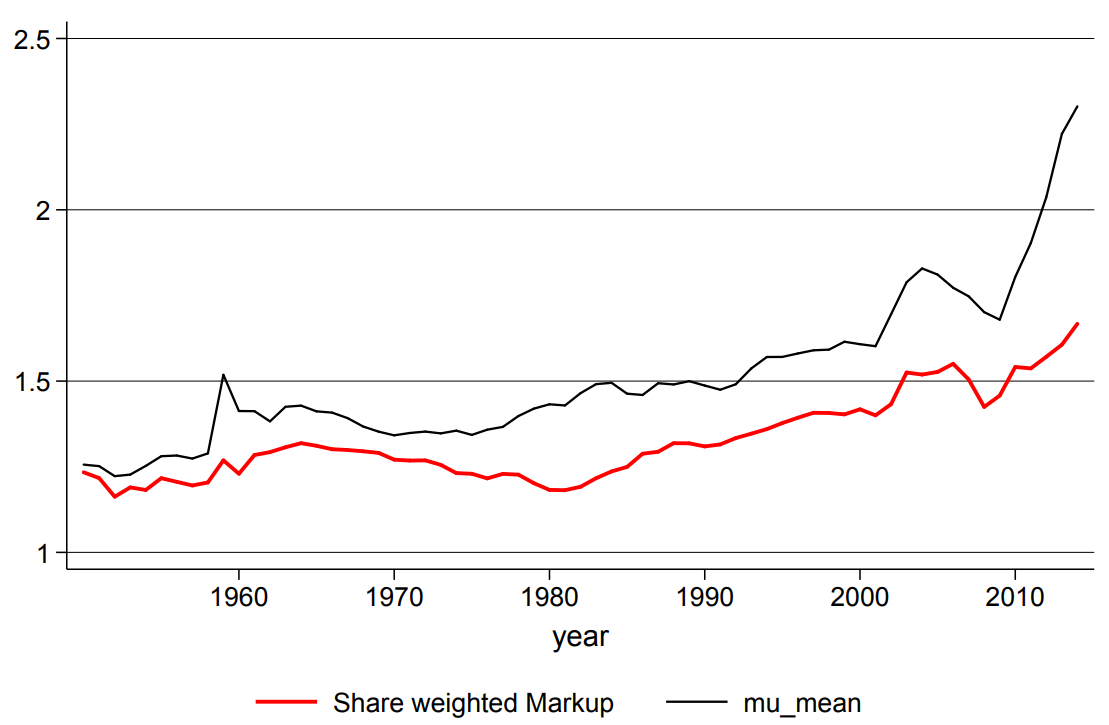
\includegraphics[width=0.8 \textwidth]{unweighted_markups.PNG}
    \caption{Unweighted versus weighted markups (Figure 2(a) from \cite{deloecker2017rise})}
    \label{fig:unweighted}
\end{figure}

But smaller firms indeed charge higher markups than big firms in the \textit{Compustat} sample. The correlation between firm size and markups \textbf{across sectors} is negative. What can salvage the Cournot and superstar firm predictions is large heterogeneity of firm distribution in different sectors. This is indeed what De Loecker and co-authors observe, and this generates a positive correlation between markups and firm size \textbf{within sectors}.\footnote{Consider the following simple example: there are two firms in manufacturing, and two firms in farming, the farming firms charge markups of 2 and 1.1, and they represent 11 and 9\% of all sales in the economy respectively. In manufacturing, the biggest firm charges markups of 1.4 and the smallest 1.04, they weight 60 and 20\%.} Ultimately, the large heterogeneity of firm size and markup distributions in each sector casts doubt on how justifiable cross-sector aggregation is. Explaining the sector-specific differences in forces shaping competition would have helped the reader to make sense of some surprising results: for instance AT\&T and Apple--two usual suspects in this high markup story--have lower markups than the weighted average in recent years. A firmer theoretical grounding of the paper could have put these findings in perspective.\\

%But the authors actually report in the appendix that markups are \textbf{negatively} correlated with size of sales, employment and cost of goods sold. This is a direct contradiction of the superstar firm effect. A closer look at the selection of firm markups reveal that Apple, AT\&T and Microsoft all experienced a decrease in markups. In the NBER working paper version of the paper, they document that markups are negatively correlated with size across industries, but positively correlated with size within. This highlights again the importance of sector heterogeneity. This seems to be an important characterisation of their finding and I believe it would have deserved more discussion in the body of the paper. \\

%\subsection*{Precision of the measure of markups} One suspects that these measures of markup are very volatile, as seen from the decomposition of aggregate markups


\subsubsection*{2. Inclusion of marketing and management costs} A key critique of the paper's methodology concerns the omission of marketing, advertising and administrative costs in the variable cost expenditure term. This point has been initially made by \cite{traina2018aggregate} who notes that if marketing and management costs are included in variable costs, the increase in markups disappear. To see this, one can refer to the measure of markups used by \cite{de2019rise} (the appendix provides a summary of the derivation):
$$\mu_{i t}=\epsilon_{i t}^v \frac{P_{i t} Q_{i t}}{P_{i t}^{V} V_{i t}}$$

De Loecker and co-authors do not include administrative expenses either in the denominator or in the production function used to estimate the output elasticities $\epsilon_{i t}^v$. As a result, the ratio of sales to variable inputs and the elasticity are overestimated. Leading to an upward level shift of markups. Furthermore, the share of administrative costs in total costs has increased since the 1950s, so De Loecker and co-authors are not only overestimating the level of markups but also their upward trend. Figure \ref{fig:traina} below shows ``Costs of Goods Solds'' (COGS), the measure of variable costs used by \cite{de2019rise} as a share of total expenditures (left) and how aggregate markups change when using total expenditure instead (right).\\ 

\begin{figure}[h!]
    \begin{tabular}{cc}
        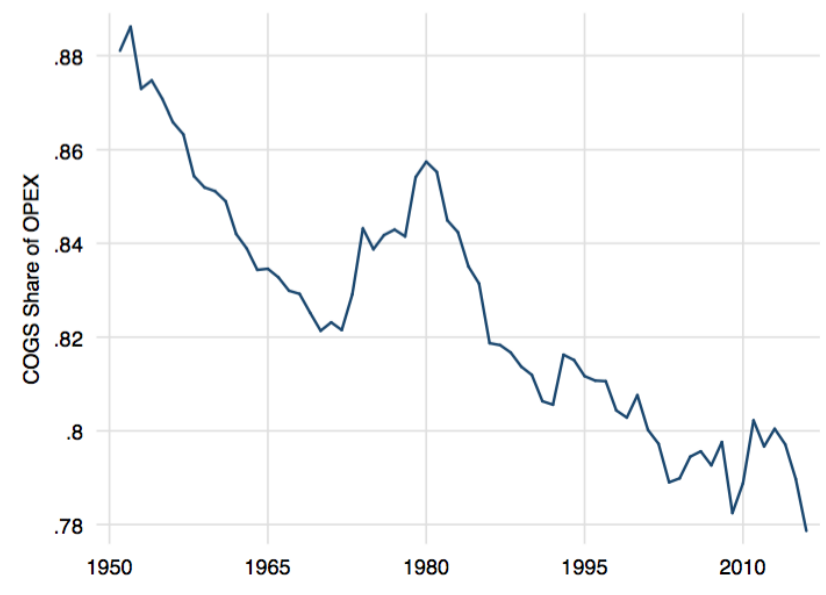
\includegraphics[width=0.48 \textwidth]{shareCOGS.PNG} & 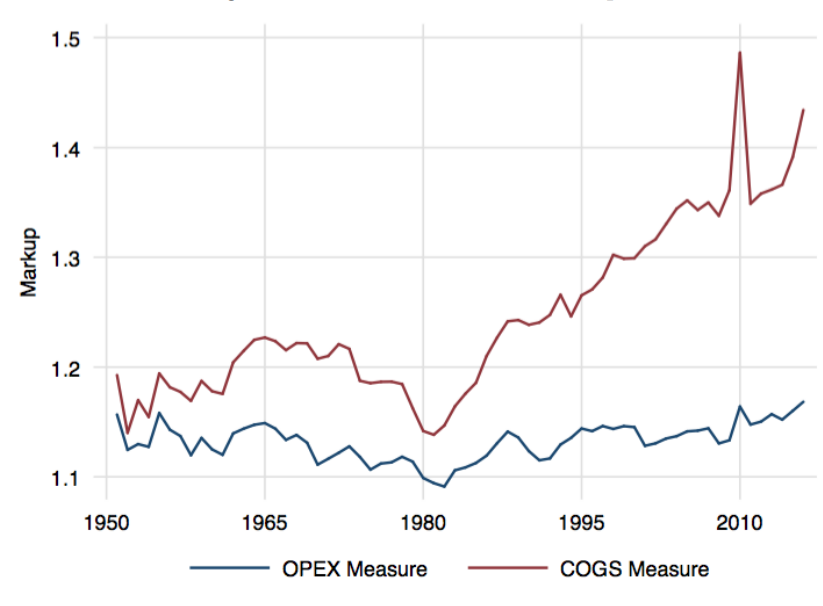
\includegraphics[width=0.48 \textwidth]{markups.PNG} \\ 
    \end{tabular}
\caption{Share of ``Cost of Goods Sold'' in total expenditures (left)  \& resulting markups (right) (figures 2 and 4 from  \cite{traina2018aggregate})}
\label{fig:traina}
\end{figure}

\cite{de2019rise} are effectively abstracting from all the costs that are necessary to bring the product to the consumer. The justification of this  assumption boils down to what makes a cost variable or fixed. By abstracting from administrative expenses altogether, the authors assume they are fixed costs. This assumption would have deserved more justification and the authors somewhat unconvincingly and partially address it in the paper.\footnote{They argue that the measure of markups that includes administrative costs is not capturing markups but something closer to operation profit rate.}

%In a response to various comments raised by their initial work \citep{de2018some}, the authors defend their choice of COGS as a measure of variable input by arguing that SG\&A reflects fixed costs and thus does not adjust immediately. R\&D expenditure, marketing and advertising are long-term endeavour and they should not be used when calculating output elasticities or the ratio of variable costs to total sales. They argue that his measure of markups is not capturing markups but something closer to operation profit rate. According to them, this requires us to assume that overhead costs adjust flexibly and are perfect substitutes with traditional variable inputs in COGS. This assumption does not seem ill-founded to me. Increasing sales can be achieved through larger input quantities or more lreliable delivery, more aggressive marketing, etc. In particular, these inputs in the production process are more substitutable the large time horizon one considers.\\

%Importantly, this measure of markups lead to an unambiguous positive relationship between markups and firm size, across sectors.\\

%\subsubsection*{Composition of the \textit{Compustat} sample} The authors document a positive relationship between markups and firm size within industries. But this source of changes in markups is not presented in the paper. While within firm variation in markups is shown, tyhe authors do not explain if the overall composition of the \textit{Compustat} sample changes over time

%\subsection*{Important contribution in the measurement of firm-level markups} The Herfindalh-Hirschman Index (HHI) is inadequate to study markups over time and space as it depends on the definition of a market. \cite{de2019rise} \\


%Furthermore, the different ways in which output elasticities are computed cast doubt on the comparability of the results.\\

\subsubsection*{3. Representativeness and composition of the Compustat sample} 

\textit{Compustat} only consists of publicly traded firms. This has important implications when considering the welfare consequences of high markups. Back-of-the-envelope calculation can help us get an idea of the magnitude of the phenomenon De Loecker and co-authors are documenting. Firstly, \cite{davis2006volatility} finds that publicly traded firms represent only 1/3 of US total sales and employment, excluding self-employed and farm workers. Secondly, one of the most striking results of the paper is that markups are only increasing for the top 10\% of firms in the markup distribution (Figure 3(b) in the paper). Lastly, 1/3 of this increase in markups is actually due to larger overhead costs and not market power. Assuming that a representative consumer shops a basket of goods reflecting the revenue shares of companies, the three facts mentioned above indicate that the rise in markup due to market power pertains to $10\% \times \dfrac{1}{3} \times \dfrac{2}{3} = 2.2\%$ of consumers' purchases.\\

To show that the rise of markups is an economy-wide trend, the authors provide some helpful comparisons of their measure of markups estimated on various Censuses of firms. Unfortunately, the results are not entirely convincing. The authors estimate markups that go up to 40 times the marginal cost for the 90\textsuperscript{th} percentile of retail firms (Figure 6 in the paper). Instead of strengthening their results, this questions the validity of their method. Moreover, the downward trend in the wholesale sector directly contradicts their earlier analysis.



%Using a re-weighting of the publicly listed firms in \textit{Compustat} to build a representative sample of the American economy, \cite{traina2018aggregate} finds that markups are flat or even decreasing over time.\\


%\subsection*{Inconsistency between the estimated markups and implied profit rates} See critique from \cite{basu2019price} and response in paper (\hl{Not that interesting}).\\


%\subsection*{Comparison with other estimates in the literature} This section (6.5) is too short and would have benefitted from a longer discussion in the paper. This paper is first and foremost methodological, so the macroeconomic implications could have been shortened. More space for robustness checks and comparison would have been helpful.\\


%\subsection*{Comparison with other methods} The method is relatively new, and the cost-minimisation assumption is not entirely standard. Most importantly, if a firm is minimising costs taking input prices as given, this implicitly assumes that firms do not have any wage-setting power. Recent evidence from the US economy show that this assumption may not be totally innocuous \citep{council2016labor}.\\

%\subsection*{Assumption of fixed marginal cost for all inputs} \cite{de2019rise} assume that marginal costs are constant across variable inputs. As marginal cost must be the same along each margin, it enables them to use all expenditures on inputs, including labour and intermediate materials, to calculate output elasticities.


\subsection*{Theoretical concerns}

\subsubsection*{The fall in labour share} High-markup firms tend to have lower labour shares. This follows mechanically from the firm's optimisation problem that higher markups lead to lower expenditure on inputs like labour. Combining this observation with their increased sales-weight in the US economy can allow us to make sense of the secular decline in the labour share. This echoes the findings of \cite{autor2019fall} and \cite{kehrig2017growing}. The authors argue that increased market power is the cause behind the rise of markups and the diminution of the labour share of income.\\

The only issue with this argument is that the timing of their rise in markups does not correspond 1-to-1 to that of the fall in the labour share. The labour share drops relatively sharply in the 2000s but is rather stable before, yet their markup measure increases from the 1980s onward. Figure \ref{fig:labourShare} shows the fall in the labour share in the United States.

\begin{figure}[h!]
    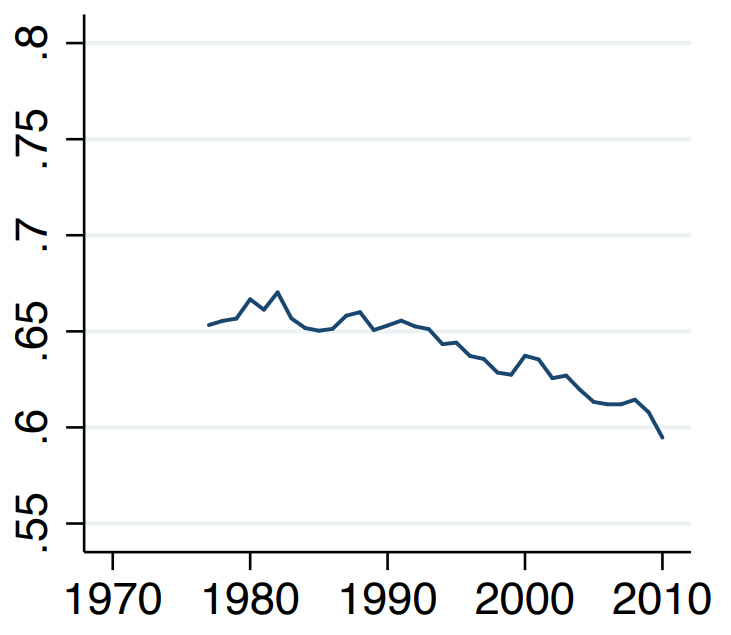
\includegraphics[width=0.5 \textwidth]{labourShare.PNG}
    \caption{Ratio of labour compensation to gross value-added in the US (Figure 1 from \cite{autor2019fall})}
    \label{fig:labourShare}
\end{figure}

%\subsection*{Implications for the fall of the labour share} One of the most interesting implication of the empirical findings documented in the paper is the relationship between the rise of aggregate markups and the fall of the labour share.\\

%\subsection*{The role of globalisation} Tax evasion. maybe market power has increased because...\\
%Also, some American sectors such as manufacturing are fiercely competing with China, yet the authors report an increase of markups in all industries. It is hard to square evidence from trade with their thesis.\\


%\subsection*{Explaining the great moderation} The rise of markups documentaed by the authors could explain the apparent stagnation in American productivity growth since the 1970s. A firm with higher market power can charge higher prices and sell lower quantities, moving up the demand curve. This leads measured GDP to be lower. Hence GDP growth will be constantly lower is markups are steadily increasing.\\

%\subsection*{Profits of US multinationals as a flawed measure} See here https://marginalrevolution.com/marginalrevolution/2017/07/american-corporate-profits-really-high.html

%\subsection*{Problem when new products are introduced} A lot of firms such as Google and Facebook have actually lowered margins compared to the status quo ante.

%\section*{Suggested extension}

%\subsection*{Input-output linkages}

%Important economic question, spurred by the rise of firm profit shares, in particular for large firms.\\

%\subsection*{Linking higher markups to innovation rates} Higher fixed costs and higher markups mean that taking the incumbent's position as a market leader has become a more profitable goal. Given the richness of the \textit{Compustat} data, it is a shame that the authors did not relate their markup measure to innovation. two questions would be interesting to address: does innovation by incumbent decrease with higher markups? And does innovation by challenging firms increase? An effort in this direction is the works of \cite{aghion2008competition} and \cite{aghion2019theory} who find that there is an inverted U-shape relationship between productivity growth and markups.

\section*{Conclusion}

Ultimately, this article is a rather convincing piece of evidence that market power is rising in the American economy. As this question is multifaceted and hard to assess, the evidence documented by De Loecker and co-authors needs to be considered along with other bits of evidence that market power is rising. This includes increased market concentration \citep{autor2017concentrating}, rising profits \citep{barkai2019declining}, decreased investment \citep{gutierrez2017investment}, and large decreases in labour share in concentrated markets \citep{azar2017labor}.\\

The novelty of the methodology pioneered by the authors is what makes both the strengths and the weaknesses of the paper. It would be helpful to see more research being done using this approach on better quality data to confirm its findings. The timeliness of the paper and the discussion it has already generated make it a landmark piece of research.

\newpage

\bibliographystyle{ecta}
\bibliography{bibliography}

\newpage

\section*{Appendix}

\subsection*{Summary of the method}

%The Industrial Organisation literature has relied on a two-step method--the ``demand approach''--to empirically estimate markups: first, estimate consumer demand, then model how firm compete, and finally combine these insights to estimate how far above marginal costs can prices. This approach is demanding in terms of data, and does not scale well to study larger macroeconomic questions.\\

The authors rely on a method pioneered by \cite{hall1988relation} and refined by \cite{de2012markups}: the \textbf{production approach}. It consists in backing out markups from the variation in the share of a variable input expenditure to total revenue and the output elasticity of this input.\\

%there are three approaches to estimating markups:
%\begin{itemize}
%    \item \textbf{Relying on observed profit margins}. This is straightforward to implement but requires to equate marginal and average costs.
%    \item \textbf{The demand approach from IO}.
%    \item \textbf{The production approach}. This method only requires the specification of a production function.
%\end{itemize}

To compute markups, researchers need to get an estimate of marginal costs. When using the production approach, this is made possible by stating the problem of the firm as a cost-minimisation one.\footnote{The cost-minimisation assumption is not entirely standard. Most importantly, if a firm is minimising costs taking input prices as given, this implicitly assumes that firms do not have any wage-setting power. Recent evidence from the US economy show that this assumption may not be totally innocuous \citep{council2016labor}} The marginal cost thus naturally appears as the Lagrange multiplier in the cost-minimisation problem. Manipulating the first order condition of the firm allows one to express markups as a function of the revenue share of variable inputs and the output elasticity of variable input: $$\mu_{i t}=\epsilon_{i t}^v \frac{P_{i t} Q_{i t}}{P_{i t}^{V} V_{i t}}$$

A crucial component of this formula is thus the output elasticity $\epsilon_{i t}^v$. These elasticities are sector- and time-specific. In this paper, they are estimated using a variant of the technique introduced by \cite{olley1996dynamics} to estimate production functions without imposing the assumption of constant return to scale. \\

A contentious part of the paper pertains to how firm-level markups are being aggregated. they calculate aggregate markups as

$$ \mu_{t}=\sum_{i} m_{i t} \mu_{i t} $$ 

where $m_{it}$ is the weight of firm $i$ at $t$. The authors use the sales share of firms as weights. But they show that if input weights are used instead, the rise of markup still holds, but the rise is less pronounced. This result is consistent with the theory: if market power increases, quantities sold and inputs used decrease, but total sales increase through higher prices. Thus using input shares understate the magnitude of markups.\\

%\section*{Minor Comments}

%\subsection*{Cross-validation of the measure of markups} Because the methodology used by the authors is so cutting edge and has rarely been used before, we may be worried that it captures something else than market power. The authors provide helpful cross-validation of this measure by comparing it to other suggestive measures of market power: profit rates, market value as a share of sales, dividends. This supporting evidence is helpful in making the case that higher markups are not simply a response to higher fixed costs.\\

%Their figure 8 reports profits since the 1980s and the trend is clearly increasing. They report total profit rates since the 1960s in the appendix and one can clearly see that they spike in the 1970s. The authors explain this by lower capital expenditures in a period of high inflation. They show the gross profit time series (without substracting capital expenditure) and find that there is no spike in profits in the 1970s. Yet gross profits are as high in the 1960s as in the 2000s, two periods that the authors have opposed throughout the paper. This part of the paper is not entirely convincing.\\

\end{document}

%------------------------------------------------------------------------------
% End of journal.tex
%------------------------------------------------------------------------------
